\documentclass[10 pt]{report}

\pagenumbering{arabic}

\usepackage[a4paper,top=2.5cm,left=2.5cm,right=1.5cm,bottom=2.5cm]{geometry}
\usepackage{graphicx}
\usepackage{amsmath,amssymb}
\newcommand{\tarc}{\mbox{\large$\frown$}}
\newcommand{\arc}[1]{\stackrel{\tarc}{#1}}
\newcommand{\norm}[1]{\left|\left| #1 \right|\right|}
\newcommand{\on}[2]{\Big|_{#1}^{#2}}
\newcommand{\inn}[1]{\langle #1\rangle}
\newcommand{\LO}[1]{\mathcal{L}(#1)}
\newcommand{\img}{\mathrm{Img }\ }
\newcommand{\pr}[1]{\left(#1\right)}
\newcommand{\R}{\mathbb{R}}
\newcommand{\C}{\mathbb{C}}
\newcommand{\qed}{\hfill $\blacksquare$}
\newcommand{\ped}{\hfill $\square$}
\newcommand{\size}[1]{\left|#1\right|}
\newcommand{\N}{\mathbb{N}}
\newcommand{\conj}[1]{\overline{#1}}
\newcommand{\spn}[1]{\mathrm{span}\left(#1\right)}
%\pagestyle{empty}
\graphicspath{./}

\usepackage{setspace}

\linespread{1.3}
%\usepackage{multirow}
\usepackage{amsfonts}

\usepackage{xcolor}
\usepackage{hyperref}
\usepackage{float}
\usepackage{enumerate}

\hypersetup{colorlinks=true,linkcolor=blue,urlcolor=blue}


\usepackage{xepersian}

\settextfont[]{XB Niloofar}
\setdigitfont{Yas}
\setlatinmonofont[]{Times New Roman}

\begin{document}
	%$$\includegraphics[width=2.5cm]{logo.png}$$

\begin{center}
	\vspace*{-2 cm}
به نام خدا\\
%\vspace*{0 cm}

\large\textbf{ 
امتحان پایانترم بهینه‌سازی محدب
}
	
	
\end{center}
کیارش بنی‌هاشم \hspace*{0.3 cm}  \small{۹۶۱۰۹۹۶۳} \hfill{بهار ۱۳۹۹}\\
\vspace*{-0.5cm}
\hrulefill
\vspace*{0.5cm}
	\begin{enumerate}
	\item دقت کنید که یک مجموعه نامتناهی است اگر و تنها اگر 
ماکسیمم قدر مطلق درایه‌هایش نامتناهی باشد. این عملا بدیهی است زیرا اگر تعریف نامتناهی را نامحدود بودن نرم $l2$ بگیریم، چون در فضای $n$بعدی، نرم $l2$ بزرگتر مساوی ماکسیمم درایه است  (طبق فیثاغورث یا حتی نامساوی مثلث) و همچنین از
$\sqrt{n}$
برابر نرم $l_\infty$ کمتر است (طبق فیثاغورث)، می‌توان این فرض را کرد.\\
در نتیجه نامتناهی بودن، معادل با این است که حداقل در یکی از $2n$ جهت مختصات، برنامه نامتناهی باشد. معادلا می‌توان برای هر $2n$ حالت از بردار 
$v=(-1)^{k}e_i$،
سعی کنیم که مقدار را بیشینه کنیم. یعنی می‌توان این $2n$ برنامه را حل کرد و دید که آیا حداقل یکیشان نامتناهی است یا نه
\[
maximize v^Tx\]\[
s.t. \quad Ax \le b \land Cx = d
\]
اما چون گفته شده ۱ برنامه، همه‌ی این‌ها را با هم قاطی می‌کنیم. یعنی به شکل زیر (در زیر، $V$ همان مجموعه‌ی $2n$ برداری است که از در نظر گرفتن خود بردار‌های مختصات و منفی‌شان به دست می‌آید.)
\[
maximize \sum_{v \in V} v^Tx_{v}\]\[
Ax_{v} \le b \land Cx_{v} = d
\]
دقت کنید که برای هر کدام از $2n$ حالت مختلف، یک متغیر $n$‌تایی جدید گرفته‌ایم. ادعا می‌کنیم مثبت بی‌نهایت بودن جواب این برنامه معادل با نامتناهی بودن 
\lr{polyhedron}
است. اگر 
\lr{polyhedron}
نامتناهی باشد، یکی از مختصات‌ها به مثبت بی‌نهایت میل می‌کند. در نتیجه 
$x_{v}$
متناظر با همه‌ی دیگر را یک نقطه‌ی ثابت می‌گیریم و در نتیجه در تابع هدف، این جملات ثابت می‌مانند. 
$x_{v}$
مربوط به این مختصات اما چون می‌تواند به بی‌نهایت میل کند، $lp$ هم می‌تواند به مثبت بی‌نهایت میل کند.\\
با توجه به این که این راه حل رو میشه تو $cvx$ زد طوری که کار کنه، سراغ این که دوگانش رو دربیاریم و یه جوری ربط بدیم به این که این نامتناهی اگر و تنها اگر اون 
\lr{feasible}
باشه و اینا نمی‌رم. همچنین چون با همین حالت میشه تو $cvx$ زد، سراغ این که فرم بلوکی ماتریس $A'$ جدید که گنده‌تر شده رو بنویسم هم نمی‌رم.\\
ابعاد
$lp$
اما خب به وضوح خیلی خوب نیست و اگر $n$ تا $lp$ جدا می‌زدیم فکر کنم بهتر میشد چون عملا من هم همین کار رو کردم و در این حالت صرفا امید به $cvx$ و ایناست که خودشون ببینن که $A$ جدید اسپارسه
	\pagebreak
	\item با استفاده از محاسبه‌ی هسین مساله را حل می‌کنیم. همچنین برای سادگی به‌جای نمادگزاری مساله، از
$x^\alpha y^\beta$
استفاده می‌کنیم.
\[
\nabla f = \begin{bmatrix}
	\alpha x^{\alpha - 1}y^{\beta}\\
	\beta x^{\alpha}y^{\beta - 1}\\
\end{bmatrix}
\implies
H = x^{\alpha - 2}y^{\beta - 2}\begin{bmatrix}
\alpha (\alpha - 1)y^2 & \alpha \beta xy\\
 \alpha \beta xy & \beta (\beta - 1)x^2\\
\end{bmatrix}
\]
حال دقت کنید که ضریب پشت ماتریس همواره مثبت است. پس برای بررسی $H$ باید دترمینان آن و نیز ضرایب روی قطر را بررسی کنیم. \\
\begin{enumerate}
	\item 
	$H$ مثبت‌نیمه‌معین است اگر و تنها اگر
	\[
	\alpha (\alpha - 1) \ge 0 \land \beta (\beta - 1) \ge 0 \land x^2y^2\alpha \beta (1 - \alpha - \beta) \ge 0
	\]
	در نتیجه اگر 
	$\alpha, \beta > 0$
	باشند که ممکن نیست چون که 
	باید هر دو حداقل ۱ باشند و در نتیجه نامساوی سوم درست نخواهد بود.\\
	اگر هر دو منفی باشند (منظور نامثبت)، مشکلی نداریم چون که نامساوی‌های برقرارند. پس اگر هر دو نامثبت باشند تابع محدب است.
	اگر یکی مثبت و دیگری نامثبت باشد، مثلا $\alpha$ مثبت باشد، در این صورت
	\[
	\alpha (\alpha - 1) \ge 0 \implies \alpha \ge 1, \quad \beta(1 - \alpha - \beta) \ge 0 \implies
	\beta \ge 1 - \alpha 
	\]
	از طرفی دقت کنید که اگر 
	$\alpha \ge 1, \beta \ge 1- \alpha$،
	هر ۳ نامساوی برقرارند. پس یک حالت هم این است که 
	$\alpha\beta \le 0, \alpha + \beta \ge 1$.
	شکل مورد نظر در 
	\ref{fig2:convex}
	آمده است.
	\item 
برای دو شرط اول باید داشته باشیم
\[
\alpha(\alpha - 1) \le 0\land  \beta(\beta - 1) \le 0  \implies1 \ge  \alpha, \beta \ge 0
\]
همچنین  برای شرط سوم باید داشته باشیم
\[
1 - \alpha - \beta \ge 0 \implies \alpha + \beta \le 1
\]
پس مقعر بودن معادل است با
\[
\alpha, \beta \ge 0 \land \alpha + \beta \le 1
\]
شکل مورد نظر در 
\ref{fig2:concave}
آمده است.
\begin{figure}[H]
	\centering
	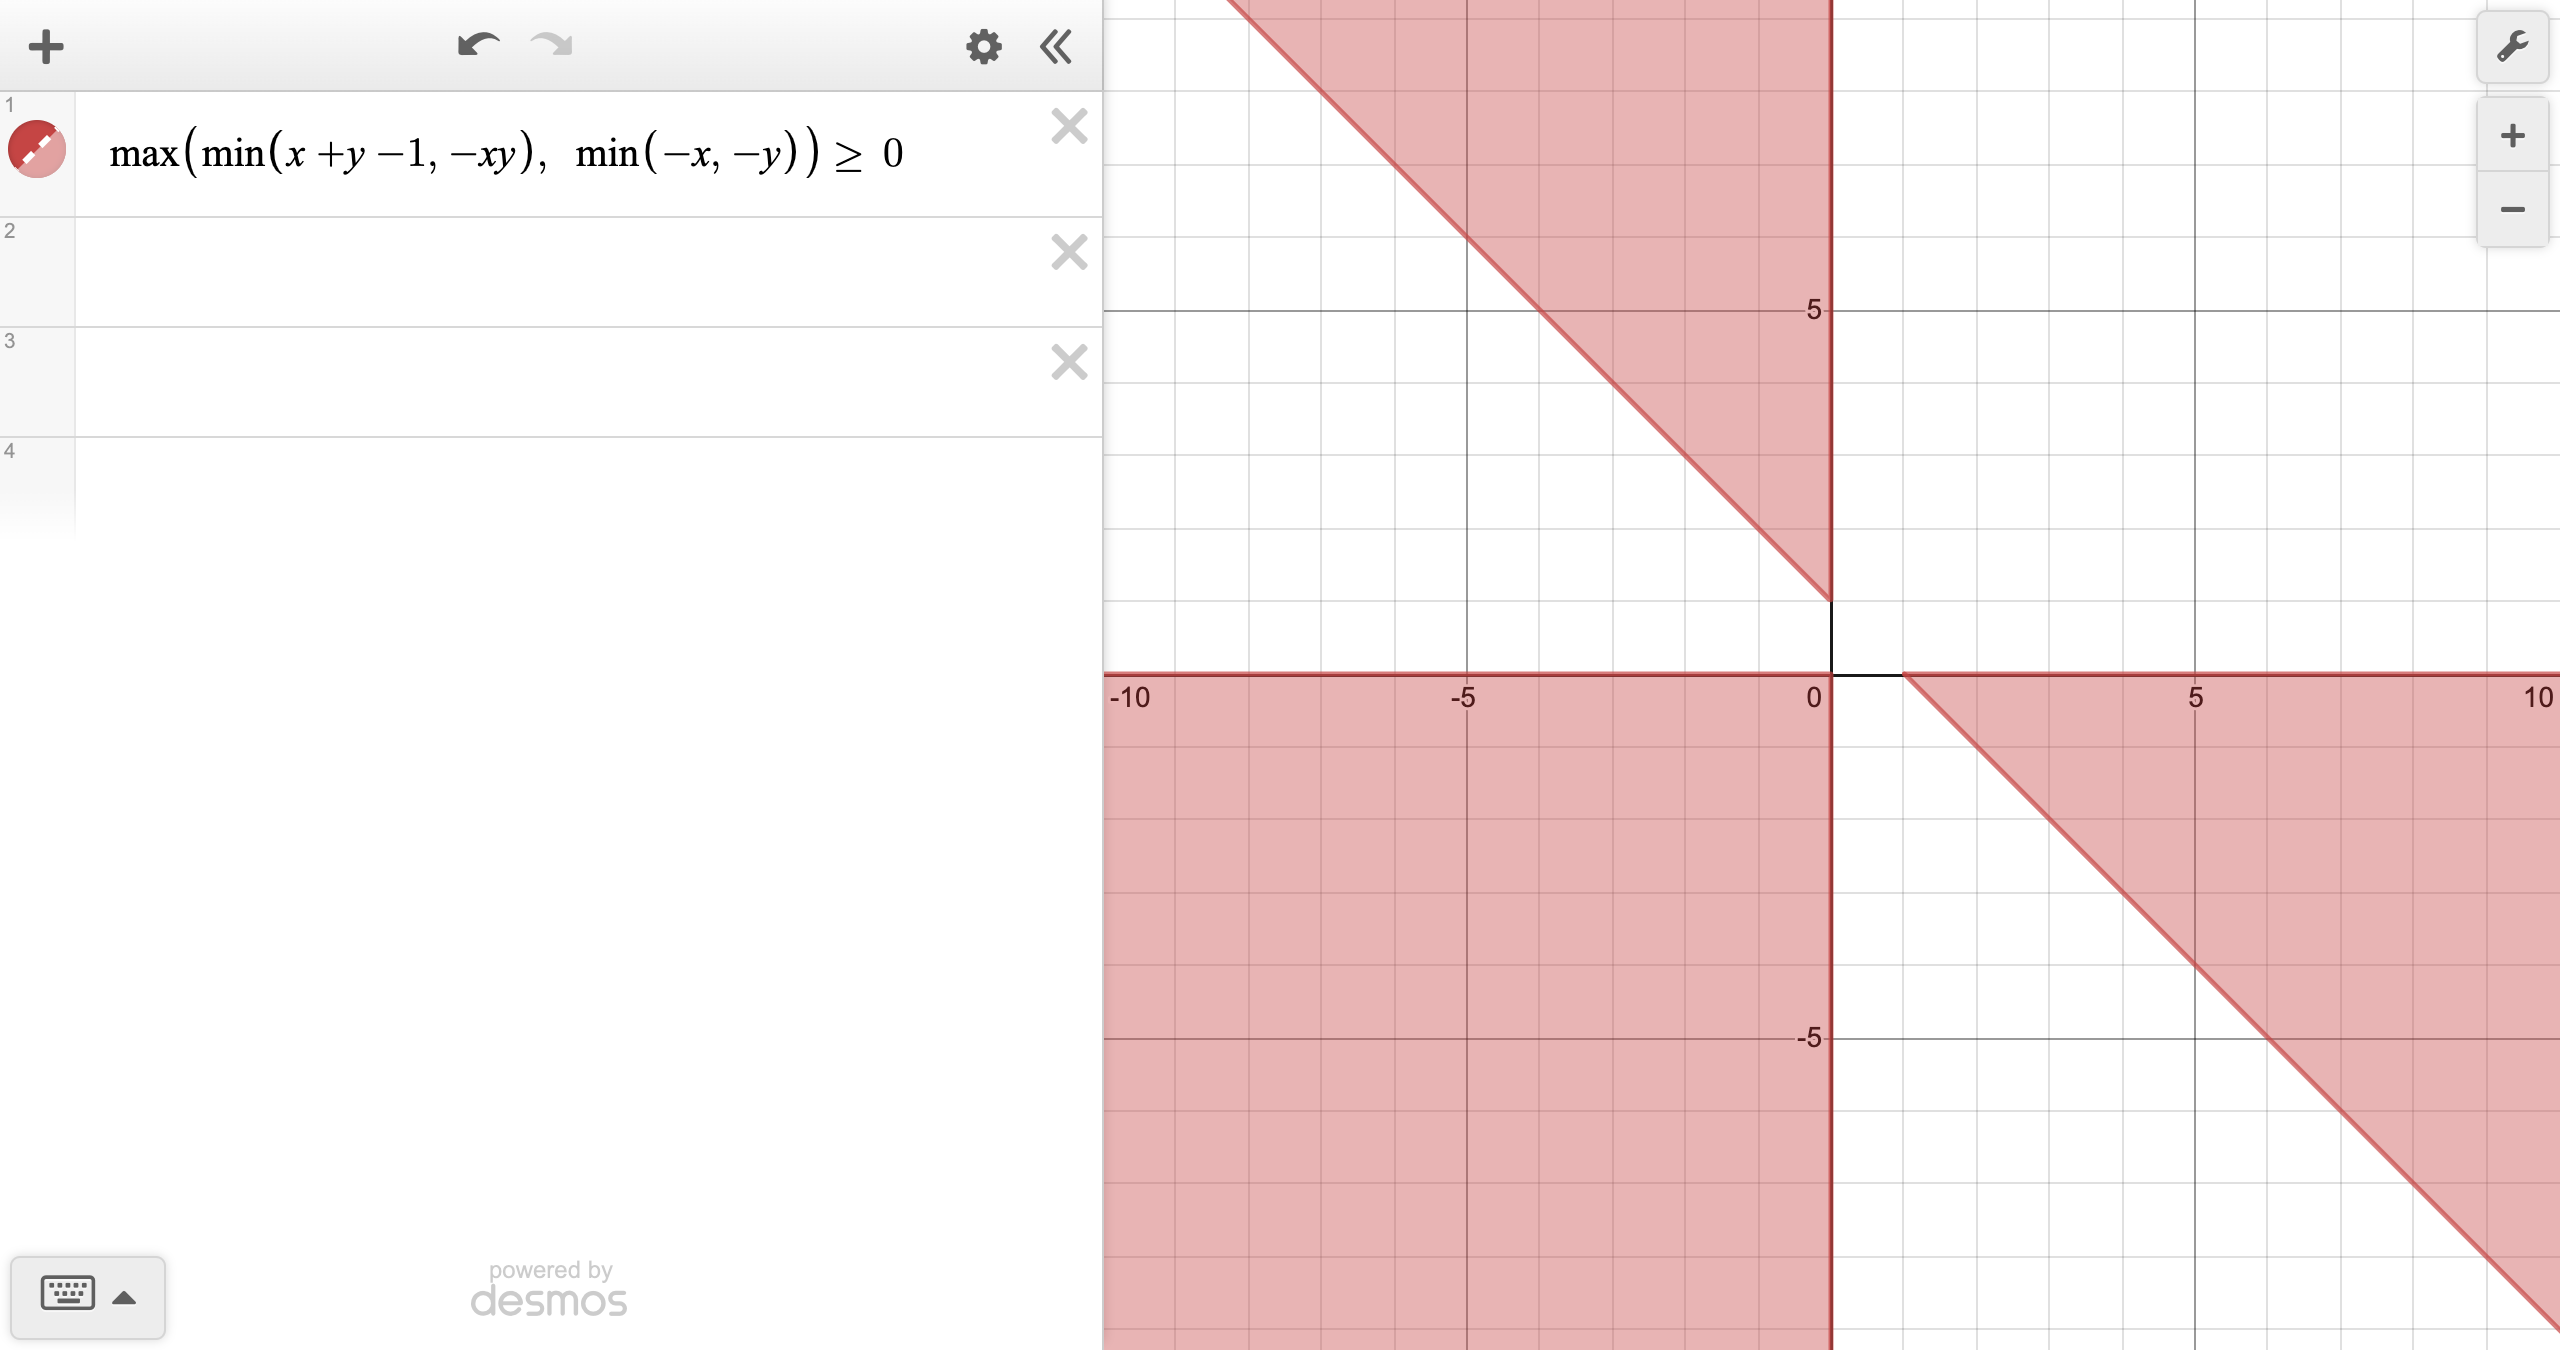
\includegraphics[width=0.9\textwidth]{convex}
	\caption{شکل سوال ۲ الف}
	\label{fig2:convex}
\end{figure}
\begin{figure}[H]
	\centering
	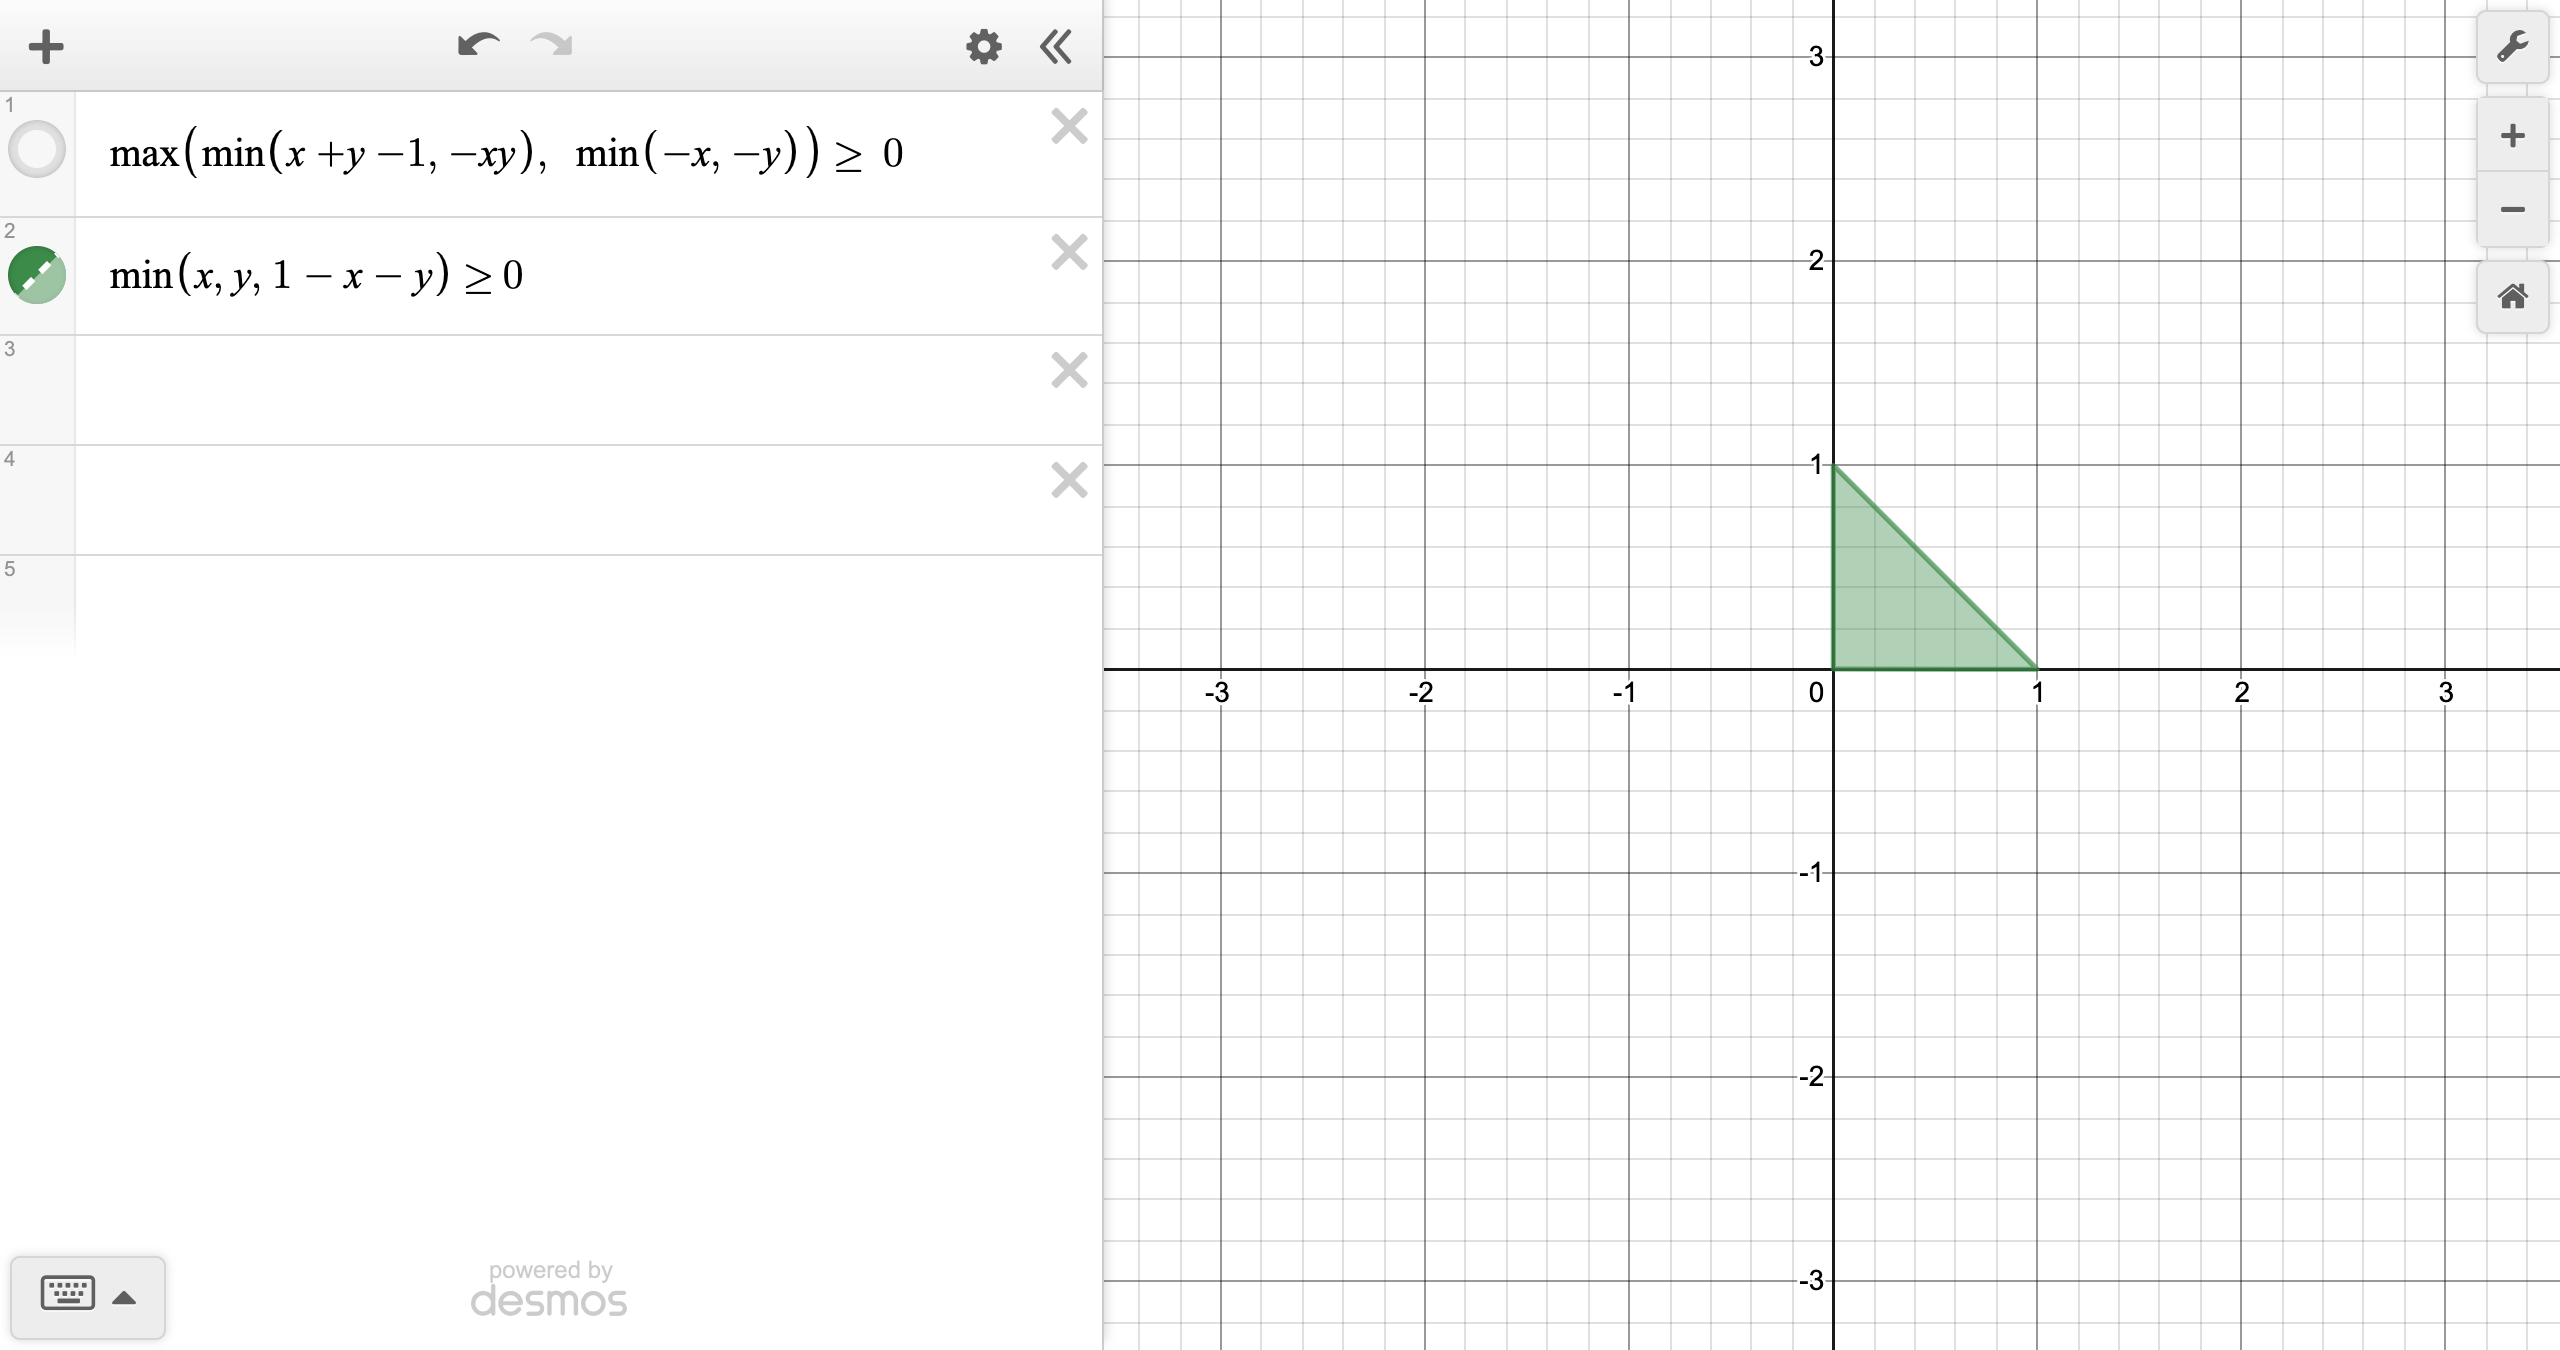
\includegraphics[width=0.9\textwidth]{concave}
	\caption{شکل سوال ۲ ب}
	\label{fig2:concave}
\end{figure}
\end{enumerate}
حال به حل بخش امتیازی می‌پردازیم. به این منظور، دقت کنید که هسین روی قطر برابر است با
\[
(\prod x_i^{\alpha_i} )\frac{\alpha_i (\alpha_i - 1)}{x_i^2}
\]
و خارج از قطر برابر است با
\[
(\prod x_i^{\alpha_i} )\frac{\alpha_i \alpha_j}{x_ix_j}
\]
که چون 
$(\prod x_i^{\alpha_i} )$
مثبت است، می‌توان آن را در نظر نگرفت. با این توصیفات، به حل مساله می‌پردازیم. 
\textbf{ابتدا مقعر بودن و سپس محدب بودن را بررسی می‌کنیم}
\begin{enumerate}
	\item 
اولا دقت کنید که اگر 
$\alpha_i < 0$،
درایه‌ی $i$‌ام روی قطر مثبت خواهد بود. در نتیجه قطعا مقعر نیست. پس
$\alpha \ge 0$.
حال برای هر $v$ دلخواه باید داشته باشیم.

\begin{equation}
\forall v \in R^n : \sum v_i^2\frac{\alpha_i^2 - \alpha_i}{x_i^2} + 2\sum_{i \ne j} v_iv_j\frac{\alpha_i\alpha_j}{x_ix_j} \le 0 \iff 
(\sum v_i\frac{\alpha_i}{x_i})^2 \le \sum \alpha_i\frac{v_i^2}{x_i^2}
\label{eq2:1}
\end{equation}

اگر که داشته باشیم
$\sum \alpha_i \le 1$،
\[
RHS \ge RHS \times \sum \alpha_i = (\sum \alpha_i)(\sum \alpha_i\frac{v_i^2}{x_i^2})
\]
که طبق کوشی شوارتز از
$LHS$
بیشتر است و در نتیجه تابع مقعر است. از طرفی اگر 
\ref{eq2:1}
برای $v$ دلخواه برقرار باشد، داریم
\[
v_i = x_i \implies (\sum \alpha_i)^2 \le (\sum \alpha_i) \implies \sum \alpha_i \le 1
\]
پس تابع مقعر است اگر و تنها اگر
\[
\alpha \ge 0 \land \sum \alpha_i \le 1
\]
\item 
فرض کنید که دو تا از
$\alpha_i$‌ها
مثبت باشند. در این صورت با در نظر گرفتن تصویر روی همان دو متغیر، باید هنوز تابع محدب بماند. اما با توجه به این که در بخش غیرامتیازی ثابت کردیم که اگر محدب باشد همچین چیزی ممکن نیست، این حالت منتفی است. پس یا همه نامثبت‌اند و یا دقیقا یکی مثبت است. اگر همه نامثبت باشند، باید برای هر $v$ دلخواه داشته باشیم (بسط دادن هسین مشابه قبل است)

\begin{equation}
\forall v \in R^n : \sum v_i^2\frac{\alpha_i^2 - \alpha_i}{x_i^2} + 2\sum_{i \ne j} v_iv_j\frac{\alpha_i\alpha_j}{x_ix_j} \ge 0 \iff 
(\sum v_i\frac{\alpha_i}{x_i})^2 \ge \sum \alpha_i\frac{v_i^2}{x_i^2}
\label{eq2:2}
\end{equation}

که همواره برقرار است زیرا سمت راست نامثبت است و سمت چپ نامنفی.
اگر هم دقیقا یکی از 
$\alpha_i$‌ها
مثبت باشد و بقیه نامثبت، با قرار دادن 
$v_i=x_i$
نتیجه می‌گیریم که 
\[
(\sum \alpha_i)^2 \ge \sum \alpha_i
\]
و در نتیجه یا 
$\sum \alpha_i \le 0$،
یا 
$\sum \alpha_i \ge 1$.
در حالت اول، اگر همه‌ی
$x_i$
‌هایی که ضریبشان منفی است را یکی کنیم (یعنی یک متغیر کنیم. این کار ممکن است چون \lr{precomposition} با آفین)،
تابع باید محدب بماند. اما خب محدب نمی‌ماند زیرا الان یک 
$\alpha_i$
مثبت داریم، یک 
$\alpha_i$
نامثبت و جمعشان هم نامثبت است که در شرایط بخش غیرامتیازی صدق نمی‌کند چون در حالت یکی مثبت، یکی نامثبت، باید جمع حداقل ۱ می‌شد.\\
پس در حالت دوم هستیم و در نتیجه 
\[
\sum \alpha_i \ge 1
\]
ثابت می‌کنیم که همین شرایط کافیست. به این منظور ابتدا حالتی که 
$\sum \alpha_i = 1$
است را بررسی می‌کنیم. در این حالت، اگر فرض کنیم که 
$\alpha_n > 0$
و بقیه‌ نامثبت‌اند، می‌دانیم
$x \in R^{n - 1} \to \prod x_i^{\alpha_i}$
محدب است. در نتیجه طبق قانون پرسپکتیو، تابع زیر محدب است
\[
x \in R^{n - 1}, g(t, x) = t\prod((\frac{x_i}{t})^{\alpha_i}) = t^{1 - \sum \alpha_i} \prod x_i^{\alpha_i}
\]
که همان تابع ماست با این تفاوت که به‌جای
$x_n$
از $t$ استفاده کرده‌ایم. پس این حالت حل شد. در حالتی که 
$\sum \alpha_i > 1$
هم می‌توانیم تعریف کنیم
$g(x) = \prod x_i^{\frac{\alpha_i}{\sum \alpha_i}}$.
طبق چیزی که الان ثابت کردیم، 
$g$ محدب است.
پس چون تابع زیر محدب است (چون $\sum \alpha_i \ge 1$) و همچنین صعودی است
\[
x \in R^+, h(x) = x^{\sum \alpha_i}
\]
نتیجه می‌گیریم که تابع اصلی هم محدب است. پس برای این بخش هم ۲ حالت وجود دارد.
حالت اول این که 
\[
\alpha \le 0
\]
و حالت دوم هم این که دقیقا یکی از $\alpha_i$‌ها مثبت است و همچنین
\[
\sum \alpha_i \ge 1
\]
\end{enumerate}
	\pagebreak
	\item کد مورد نظر در زیر آمده‌است. مطابق کد، برای حل مساله از تابع
\lr{solve\_with\_removed\_index}
استفاده می‌شود که با حذف تعدادی از واکنش‌ها، مساله‌ی بهینه‌سازی را تشکیل داده و حل می‌کند. خروجی برنامه در شکل
\ref{fig:q3}
قابل مشاهده است (اعداد در این شکل آورده شده‌اند).\\
در توضیح بخش ب: مشخص است که یکی از با حذف یک دسته‌از از آزمایش‌ها، نرخ فرق چندانی نمی‌کند اما با حذف یک دسته‌ی دیگری، فرق زیادی می‌کند. علتش این است که همانطور که توضیح داده شده است، هر آزمایش به تعدادی مواد نیاز دارد که دیگری آزمایش‌ها آن را برایش فراهم می‌کنند چون $Sv=0$. در نتیجه از نتیجه‌ی حاصل می‌توان دید که یکی از آزمایش‌ها تاثیر زیادی (چه مستقیم و چه غیرمستقیم) در فراهم کردن مواد لازم برای آزمایش \lr{biomass} داشته و به شدت ضروری بوده است در حالی که‌ آزمایش دیگر این‌گونه نبوده است. به طور دقیق‌تر
\lr{transport}
بسیار ضروری بوده است چون با حذف آن نرخ بهینه به شدت کاهش پیدا کرده است.
\lstset{language=Python}
\begin{latin}
\lstinputlisting[breaklines]{../code/q3.py}
\end{latin}
\begin{figure}[H]
	\centering
	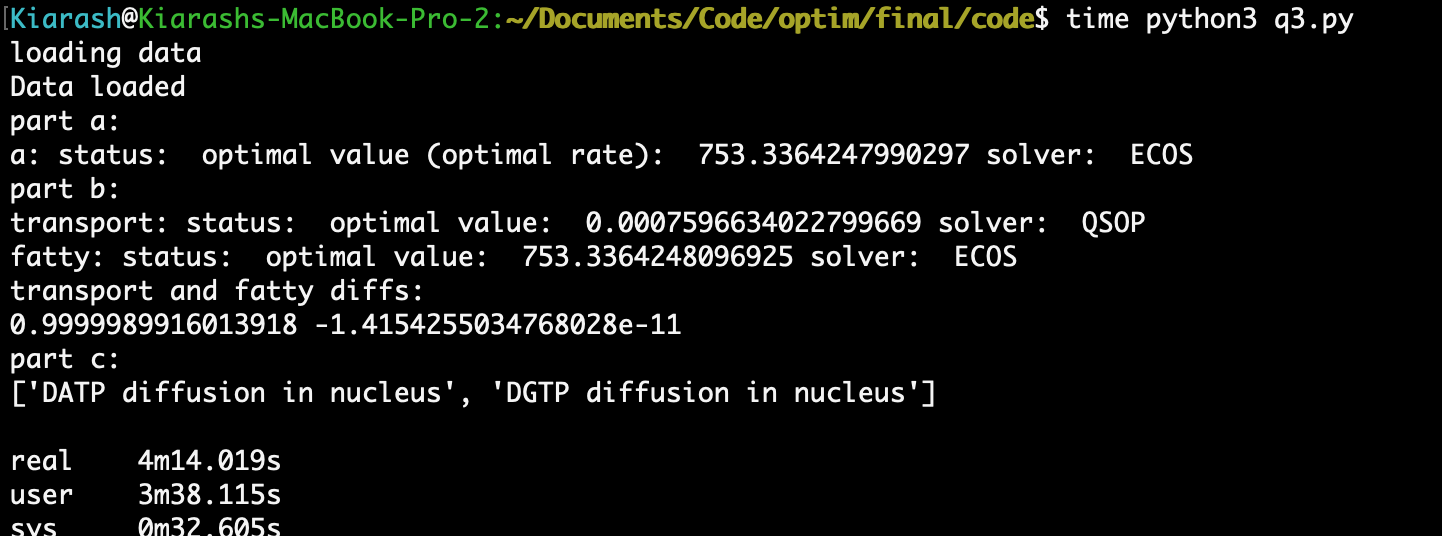
\includegraphics[width=0.9\textwidth]{q3}
	\caption{شکل سوال ۳}
	\label{fig:q3}
\end{figure}
	\pagebreak
	\item \begin{enumerate}
	\item 
صورت حکم چیزی به فرم
فلان اگر و فقط اگر بهمان است. من ثابت می‌کنم که بهمان اگر و تنها اگر فلان. دقت کنید که همان مطلب ثابت شده است و صرفا چون تشکیل دوگان از این سمت برایم راحت‌تر بود این کار را می‌کنم.\\
مساله‌ی زیر را در نظر بگیرید
\[
minmize_{\mu} \quad -c^T\mu \]\[
s.t. \quad S^T\mu \le 0
\]
این مساله به وضوح محدب است (اصلا آفین است). همچنین شرط
\lr{slater}
برقرار است زیرا اگر قرار دهیم
$\mu = 0$،
در نامساوی‌ها (که همه خطی‌اند) صدق می‌کند. در نتیجه 
\lr{strong dualtiy}
برایش برقرار است. از طرفی دقت کنید که جواب این مساله بیشتر مساوی ۰ است، اگر و تنها اگر 
بخش بهمان سوال برقرار باشد یعنی برای هر 
$S^T\mu \le 0$
بتوان گفت که 
$c^T\mu \le 0$.
همچنین همواره کمتر‌مساوی ۰ است زیرا می‌توان قرار داد
$\mu = 0$.
پس جواب این مساله ۰ است اگر و تنها اگر بخش بهمان برقرار باشد.
از طرفی با تشکیل دوگان داریم
\[
\mathcal{L} = -c^T\mu + v^TS^T\mu = (-c + Sv)^T\mu
\]
که با اینفیمم‌گیری روی $\mu$، منفی بی‌نهایت است اگر ضریب ناصفر باشد و در غیر این صورت ۰ است. پس مساله‌ی دوگان به فرم زیر است
\[
maximize \quad 0 \]\[
s.t. \quad Sv - c = 0 \land v \ge 0
\]
از طرفی جواب این مساله برابر با ۰ است، اگر و تنها اگر \lr{feasible} باشد که معادل است با این که بخش فلان مساله درست باشد یعنی
$c$
یک بردار 
\lr{thermodinamically feasible}
باشد. پس حکم ثابت شد چون ثابت کردیم که فلان معادل است با ۰ بودن جواب مساله‌ی دوگان که معادل است با 
%(این بخش همواره برقرار است یعنی کلا با \lr{slater} ثابت کردم و خیلی ربط خاصی به مساله نداشت)
%(طبق \lr{slater})
 ۰ بودن مساله‌ی اصلی که معادل است با بهمان.
\item 
فرض کنید که حکم غلط باشد. مساله‌ی زیر را در نظر بگیرید
\[
minimize \quad -t\]\[
s.t. \quad S^Tm = 0 \land m \ge t
\]
در این صورت جواب این مساله، قطعا مقداری منفی‌ای نخواهد بود زیرا اگر منفی باشد، $t$ مثبت است و در نتیجه 
$m > 0$
و همچنین
$m^TS = 0$
که حکم است و در نتیجه با فرض خلف در تناقض است. پس جواب مساله بزرگتر مساوی ۰ است. از طرفی اگر قرار دهیم
$m = 0 \land t = 0$،
به وضوح به ۰ می‌رسیم. پس جواب این مساله ۰ است.\\
مساله به وضوح محدب است (مجددا همه‌چی آفین است) و شرط 
\lr{slater}
برقرار است چون می‌توانیم قرار دهیم
$t = -1, m = 0$
(البته اگر $t=0$ قرار می‌دادیم هم اوکی بود). در نتیجه 
\lr{strong dualtiy}
داریم. مساله‌ی دوگان را تشکیل می دهیم.
\[
\mathcal{L} = -t + u^T(S^Tm) + \lambda^T(t1 - m) = 
t(\lambda^T1 - 1) + (Su - \lambda)^Tm 
\]
که با اینفیمم‌گیری روی $t, m$، برابر با منفی بی‌نهایت است اگر یکی از ضرایب ناصفر باشد و در غیر این صورت ۰ است. پس مساله‌ی دوگان به فرم زیر است.
\[
maximize \quad 0\]\[
s.t. \quad \lambda \ge 0 \land Su = \lambda \land \sum 1^T\lambda = 1
\]
چون جواب مساله‌ی اصلی ۰ بود، جواب این مساله هم ۰ است و در نتیجه
\lr{feasible}
است.
پس چون داریم
\[
Su = \lambda \ge 0
\]
طبق فرض
\[
Su = 0 \implies \lambda = 0 \implies 1 = 1^T\lambda = 0 
\]
که به وضوح تناقض است.
%\item 
%مساله‌ی زیر را در نظر بگیرید
%\[
%minimize_{v, t} \quad -t\]\[
%s.t. \quad Sv \ge t
%\]
%به وضوح محدب است چون همه‌چی آفین است. همچنین شرط
%\lr{slater}
%را دارد چون کافیست $v$ دلخواه بگیریم و 
%$t$
%را برابر با کوچکترین درایه‌ی
%$Sv$
%قرار دهیم. پس 
%\lr{strong dualtiy}
%برقرار است. از طرفی طبق فرض، جواب مساله حداکثر ۰ است زیرا اگر کمتر از ۰ باشد، 
%یک بردار $v$ داریم که 
%$Sv \ge 0
%$ اما
%$Sv \ne 0$.
%از طرفی خود ۰ هم قابل دست یافتن است زیرا کافیست قرار دهیم
%$v = t = 0$.
%پس جواب مساله ۰ است. حال دوگانش را تشکیل می‌دهیم.\\
%\[
%\mathcal{L} = -t + \lambda^T(t1 - Sv) = t(-1 + \lambda^T1) - \lambda^TSv
%\]
%که با اینفیمم‌گیری روی $v, t$، مقدار لاگرانژین منفی بی‌نهایت است اگر ضرایب حداقل یکیشان ناصفر باشد و در غیر این صورت ۰ است. پس مساله‌ی دوگان به فرم زیر است.
%\[
%maximize \quad 0\]\[
%s.t. \quad
%\lambda^T1 = 1 \land \lambda^TS = 0 \land \lambda^T \ge 0
%\]
%حال دقت کنید که 
\end{enumerate}
	\pagebreak
%	\item \begin{enumerate}
	\item بیانی که از مساله در حال حاضر داریم این است که قید‌ها به شرح زیراند
	\[
	1 \le \frac{l}{w} \le 2, \quad 10 \le w \le 20 ,\quad 20 \le l \le 30, \quad lw \ge 300
	\]
	و با توجه به این که مساحت فیلتر برابر است با
	$lw$
	و محیط برابر است با 
	$2l + 2\pi\frac{w}{2}$،
	و ارزش مساحت دوبرابر محیط است، تابع زیرا را می‌خواهیم که کمینه کنیم.
	\[
	2lw + 2l + 2\pi\frac{w}{2}
	\]
	اولا دقت کنید که قید
	$w \ge 10$
	اضافی است زیرا از
	$\frac{l}{w} \le 20$
	و
	$l \ge 20$
	نتیجه می‌شود. تعریف کنید.
	\[
	s = \sqrt{lw}
	\]
	دقت کنید که طبق قید‌های دیگر می‌توان فرض کرد کلا $l, w$ مثبتند. در نتیجه
	\[
	s^2 = lw \implies
	% l = \frac{s^2}{w}, \quad \frac{l}{w} = \frac{lw}{w^2} = \frac{s^2}{w^2}
	w = \frac{s^2}{l}, \quad \frac{l}{w} = \frac{l^2}{lw} = \frac{l^2}{s^2}
	\]
	در نتیجه قید روی 
	$\frac{l}{w}$
	را می‌توان به فرم زیر نوشت
	\[
	1 \le \frac{l^2}{s^2} \le 2 \iff 1 \le \frac{l}{s} \le \sqrt{2} \iff s \le l \le s\sqrt{2}
	\]
	قید روی $w$ هم می‌توان به فرم زیر نوشت
	\[
	w \le 20 \iff \frac{s^2}{l} \le 20
	\]
	که محدب است.\\
	قید روی $l$ هم که پابرجاست
	\[
	20 \le l \le 30
	\]
	قید روی مساحت هم به فرم زیر قابل بیان است.
	\[
	s^2 \ge 300 \iff s \ge \sqrt{300}
	\]
	با این تغییر متغیر‌ها، تابعی که باید کمینه کنیم هم به فرم زیر است.
	\[
	2s^2 + 2l + \pi\frac{s^2}{w}
	\]
	\item 
	جواب ۳۰۰ است. این کار را می‌توان با $cvxpy$ دید که کدش آمده است. همچنین می‌توان بدون آن دید (صرفا به امید نمره‌ی امتیازی و اینا نوشتم این توضیح رو). 
دقت کنید که اگر قید مساحت را در نظر نگیریم، طبیعتا هر چه $l, w$ کمتر شوند بهتر است. پس 
$l=20, w = 10$
جواب بهینه را می‌دهد. اما مشخص است که در این حالت، مساحت کافی نخواهد بود. حال که قید مساحت را اضافه می‌کنیم، اگر 
\lr{tight}
نباشد، کاملا احمقانه است زیرا معنی‌اش این است که ضریب لاگرانژ مرتبط با این قید ۰ است و در نتیجه لاگرانژین مساله، لاگرانژین مساله‌‌ی بدون قید مساحت است. در نتیجه چون این‌جا 
\lr{strong duality}
داریم (کلا مساله‌ها هم محدب‌اند و هم شرط‌ها رو میشه اکید برقرار کرد. این رو دیگه چک نکردم ولی خب قطعا میشه)، الان جواب مساله‌ی جدید همه‌ی شرط‌های $KKT$ رو برای مساله‌ی قبلی هم خواهد داشت و در نتیجه برای اون هم بهینه است که خب گفتیم نمیشه چون تو مساله‌ی قبلی حتما مساحت میشد ۲۰۰. 
\end{enumerate}
	\item \begin{enumerate}
	\item 
با توجه به قید‌ها، مشخص است که 
$l, w > 0$.
با این حساب، تعریف کنید
	\[
	l' = ln(l), w' = ln(w)
	\]
قید‌های روی 
$l, w, \frac{l}{w}$
به فرم زیر درمی‌آیند.
	\[
0 \le	l' - w' \le ln(2), \quad ln(10) \le w' \le ln(20), \quad ln(20) \le l' \le ln(30)
	\]
	همچنین قید روی مساحت به شکل زیر است
	\[
	l' + w' \ge ln(300)
	\]
	برای محاسبه‌ی هزینه هم داریم
	\[
	cost = 2lw + 2l + 2\pi\frac{w}{2} = 2e^{l' + w'} + 2e^{l'} + \pi e^{w'}
	\]
	که به وضوح محدب است.
	\item 
	کد مورد نظر در زیر آمده است (همچنین در صورت نیاز در فایل $q52$)
	\begin{latin}
		\lstinputlisting[breaklines]{../code/q52.py}
	\end{latin}
با اجرای کد می‌توان دید که سایز فیلتر ۳۰۰ است.\\
\textbf{در صورتی که استدلال بدون اجرای کد نیاز باشد:} 
اگر شرط روی مساحت را در نظر نگیریم، بهترین $l, w$ همان کمترین $l, w$ هستند یعنی مساحت ۲۰۰ که خب مطلوب نیست. اگر شرط مساحت را اضافه کنیم، قطعا باید شرط
\lr{tight}
باشد زیرا اگر یک شرط 
\lr{tight}
نباشد، ضریب دوگانش ۰ است و در نتیجه با حذف آن، طبق شرایط
\lr{KKT}
می‌توان دید که این شرط نیاز نبوده است اما خب گفتیم که این شرط نیاز است چون بدون آن جواب فرق می‌کند (دقیق‌تر از این دلیلی نمی‌بینم بنویسم چون در کلاس کلا این مطلب توضیح داده شده بود).
\end{enumerate}
	\pagebreak
	\item \begin{enumerate}
	\item 
اگر $D$ و $K$ را با بردار جایگزین کنیم (با توجه به این که قطری هستند)، داریم
$A_{i,:} = d_i + k_iG_{i,:}$.
همچنین
\[
\gamma tr(D^{-1}) + tr(K^{-1}) = \sum \frac{\gamma}{d_i} + \sum \frac{1}{k_i}
\]
با این توصیفات مساله به فرم زیر در مي‌آید.\\
\[
minimize \quad \lambda_{max}(A)
\]\[
s.t. \quad d \ge 0 \land k \ge 0\]\[
A_{i,:} = d_i + k_iG_{i,:}\]\[
\sum \frac{\gamma}{d_i} + \sum \frac{1}{k_i} \le u
\]
که با توجه به محدب بودن بزرگترین مقدار ویژه و نیز $\frac{1}{x}$، مساله به فرم مناسب درآمد.
%به وضوح مساله محدب است چون
%$\lambda_{max}$
%یک تابع محدب است زیرا می‌توان آن را به فرم زیر نوشت
%\[
%sup_{\{x: ||x||\le 1\}} \quad ||Ax||
%\]
%نوشت.
\item 

\end{enumerate}
	\pagebreak
	\item فرض کنید که می‌خواهیم بررسی کنیم که آیا $n$ نفر جا می‌شوند یا نه. باید مساله‌ی زیر را بررسی کنیم که \lr{feasible} است یا نه.
\[
0 \le x_i \le l, \quad 0 \le y_i \le w\]\[
||x_i - x_j, y_i - y_j||_{p} \ge 2\quad i < j
\]
حال دقت کنید که 
\[
||a, b||_{1} \ge k \iff 
a + b \ge k \lor a - b\ge k \lor -a + b \ge k \lor -a - b \ge k
\]
و به طور مشابه
\[
||a, b||_{\infty} \ge k \iff 
a \ge k \lor b \ge k \lor -a \ge k \lor -b \ge k
\]
نکته‌ی مهم این است که اگر علامت $a$ و $b$ را بدانیم، می‌توانیم قید بالا را به فرم آفین بنویسیم زیرا برای این که بررسی کنیم که آیا حداقل یکی از عبارات بزرگتر یا مساوی $k$ است، کافیست آن عبارتی که در آن علامت‌ها مثبتند را بررسی کنیم چون بیشترین است.\\
با این توصیفات، برای حل مساله‌ی
\lr{feasiblity}
برای $n$ نفر، فرض می‌کنیم که بر اساس $x$ مرتب‌اند به طوری که 
$x_i \le x_{i + 1}$.
برای بررسی ترتیب $y$‌ها هم، همه‌ی
$n!$
حالت ممکن را در نظر می‌گیریم. یعنی روی همه‌ی این حالات فور می‌زنیم. در هر کدام از این حالات، چون علامت را می‌دانیم، می‌توانیم برنامه‌ی محدب را تشکیل دهیم و بررسی کنیم که آیا $n$ نفر جا می‌شوند یا خیر. حال اگر جواب نهایی $T$ باشد، می‌توانیم با شروع از 1 و امتحان همه‌ی اعداد تا زمانی که به $T$ برسیم فور بزنیم 
\footnote{
	چون حل مساله برای $T$ به مراتب سخت‌تر از حل آن برای $T- 1$ است، باینری سرچ زدن کار اشتباهی است.
}
پس در کل
\[
\sum_{i=1}^{T}i! 
\]
تا باید برنامه حل کنیم. عبارت فوق از نظر مرتبه عملا $T!$ است زیرا
\[
\sum_{i=1}^{T}i! = \sum_{i=1}^{T-1}i! + T! \le (T-1)\times (T-1)! + T! \le 2T!
\]
\textbf{کران فوق برای هر دو بخش الف و ب برقرار است.}
در صورت نیاز، می‌توان کران‌هایی بر حسب $l, w$ هم داد. به طور دقیق‌تر، در حالتی که $p=1$، اگر حول هر نفر و به مرکزیت آن یک دایره‌ی
 $l_{\infty}$
 به شعاع ۱ بزنیم (در واقع همان مربع خودمان هستند)، این دوایر همدیگر را قطع نمی‌کنند زیرا اگر قطع کنند یعنی دو نقطه نزدیک‌تر از ۲ فاصله دارند. همه‌ی دوایر در مستطیل به طول و عرض
 $l+2, w+2$
 جا می‌شوند و همچنین مساحت هرکدام حداقل ۴ است. در نتیجه 
 \[
p = \infty \implies 4T \le (l+2)(w+2) \implies T \le \frac{(l+2)(w+2)}{4}
 \]
برای نمر $l1$ هم به طور مشابه همه‌چیز در همان مستطیل جا می‌شوند اما مربع‌ها مساحتشان نصف شده پس کران بالا به شکل
\[
T \le \frac{(l+2)(w+2)}{2}
\]
در می‌آید.
کد این را من نزدم چون فکر کنم در حالتی که در هر ثانیه ۱۰ به توان ۹ تا برنامه حل شوند، ۷۷ سال طول می‌کشد که تمام شود!
\end{enumerate}
	
\end{document}